\section{Khái niệm nền về xử lý công việc}

\subsection{Concurrency, parallelism, bất đồng bộ và Background Job}

\textbf{Thread (luồng thực thi)} là một chuỗi lệnh được CPU thực hiện. Một chương
trình có thể có nhiều thread. \textbf{CPU core (lõi xử lý)} là đơn vị phần cứng có
khả năng thực thi lệnh; nhiều core cho phép nhiều thread thực sự chạy cùng lúc.

\begin{itemize}
  \item \textbf{Concurrency (xử lý đồng thời)} là quản lý nhiều công việc trong cùng
  một khoảng thời gian. Các công việc có thể xen kẽ nhau, chưa chắc chạy đúng cùng
  một thời điểm.

  \item \textbf{Parallelism (xử lý song song)} là nhiều phần tính toán thực sự chạy
  cùng lúc trên nhiều CPU core. Đây là một cách thực hiện concurrency.

  \item \textbf{Asynchronous programming (lập trình bất đồng bộ)} cho phép phương
  thức tạm nhường quyền thực thi trong lúc chờ thao tác vào/ra (I/O) như mạng,
  database hoặc file. Từ khóa \texttt{await} không tự tạo thêm thread; nó giúp
  thread hiện tại quay lại xử lý việc khác cho đến khi thao tác chờ hoàn tất.

  \item \textbf{Background Job (công việc nền)} là công việc chạy độc lập với
  request, tức yêu cầu mà máy khách gửi đến server. Chẳng hạn, job dọn dữ liệu lúc
  nửa đêm có thể tiếp tục sau khi server đã trả phản hồi cho máy khách.
\end{itemize}

\figref{fig:async-io-flow} minh họa điều xảy ra tại \texttt{await}. Phương thức gửi
yêu cầu I/O rồi tạm dừng; thread đang chạy phương thức được trả về ThreadPool để xử
lý việc khác. Khi I/O hoàn tất, phần code sau \texttt{await} được xếp lịch để tiếp
tục thực hiện.

\begin{center}
\resizebox{0.84\textwidth}{!}{\begin{tikzpicture}[
  node distance=8mm and 10mm,
  every node/.style={font=\small,align=center},
  flowbox/.style={draw,rounded corners=2mm,minimum height=11mm,minimum width=28mm,thick},
  arrow/.style={-{Latex[length=2mm]},thick},
  waitarrow/.style={-{Latex[length=2mm]},thick,dashed,draw=gray!75}
]
\node[font=\small\bfseries] (threadlabel) {Thread};
\node[flowbox,fill=blue!15,draw=blue!55,right=of threadlabel] (start) {Bắt đầu\\phương thức};
\node[flowbox,fill=orange!18,draw=orange!70!black,right=of start] (send) {Gửi yêu cầu I/O\\rồi gặp await};
\node[flowbox,fill=green!15,draw=green!55!black,right=of send] (free) {Thread quay lại\\ThreadPool};
\node[flowbox,fill=blue!12,draw=blue!55,right=of free] (resume) {Tiếp tục xử lý\\sau await};

\node[font=\small\bfseries,below=16mm of threadlabel] (iolabel) {I/O};
\node[flowbox,fill=gray!12,draw=gray!65,below=16mm of send] (io) {Mạng, database hoặc file\\thực hiện thao tác};

\draw[arrow] (start) -- (send);
\draw[arrow] (send) -- (free);
\draw[arrow] (send) -- (io);
\draw[waitarrow] (io) -| node[pos=0.72,below,font=\scriptsize] {hoàn tất} (resume);
\end{tikzpicture}
}
\captionof{figure}{Luồng thực thi khi phương thức bất đồng bộ chờ I/O}
\label{fig:async-io-flow}
\end{center}

\figref{fig:concurrency-single-thread} minh họa concurrency trên một thread.
Ba công việc A, B và C đều tiến triển trong cùng một khoảng thời gian, nhưng tại
mỗi thời điểm CPU chỉ thực thi một đoạn của một công việc. Hệ thống chuyển qua lại
giữa các đoạn nên các công việc trông như cùng chạy; đây là sự xen kẽ, chưa phải
parallelism thực sự.

\begin{center}
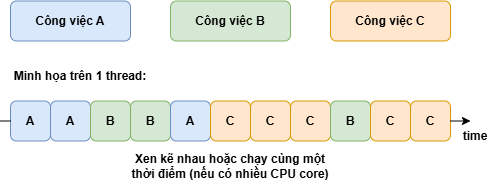
\includegraphics[width=0.64\textwidth]{../../assets/images/concurrency-single-thread.png}
\captionof{figure}{Concurrency trên một thread: các công việc được thực thi xen kẽ}
\label{fig:concurrency-single-thread}
\end{center}

Ngược lại, \figref{fig:parallelism-multiple-cores} minh họa parallelism. Các công
việc A, B và C được thực thi tại cùng một thời điểm trên các CPU core khác nhau.
Vì có nhiều phép tính thật sự diễn ra đồng thời, đây là xử lý song song chứ không
chỉ là chuyển lượt thực thi trên một core.

\begin{center}
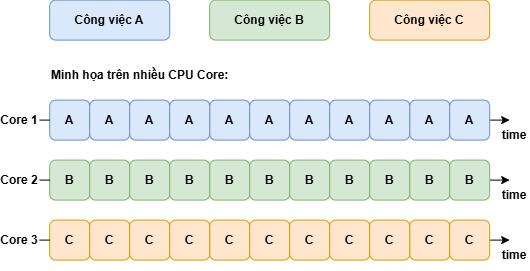
\includegraphics[width=0.64\textwidth]{../../assets/images/parallelism-multiple-cores.png}
\captionof{figure}{Parallelism trên nhiều CPU core: các công việc được thực thi đồng thời}
\label{fig:parallelism-multiple-cores}
\end{center}

Có thể hình dung bằng việc nấu ăn: một người tranh thủ chuẩn bị món khác trong lúc
chờ món đang nấu là async/concurrency; nhiều người cùng nấu các món khác nhau mới là
parallelism. Điểm khác nhau nằm ở việc công việc chỉ được sắp xếp xen kẽ hay thật sự
được thực thi đồng thời trên nhiều tài nguyên.

Trong C\#, \texttt{Task} đại diện cho một thao tác đang thực hiện hoặc sẽ hoàn tất
trong tương lai. Một Task không đồng nghĩa với một thread riêng: thao tác có thể chờ
I/O mà không giữ thread hoặc được thực thi bằng thread do .NET quản lý, tùy theo bản
chất công việc.

\subsection{Phân loại tác vụ theo tài nguyên giới hạn}

\textbf{CPU-bound} nghĩa là tốc độ bị giới hạn chủ yếu bởi thời gian CPU tính toán.
\textbf{I/O-bound} nghĩa là phần lớn thời gian dùng để chờ hệ thống bên ngoài như
database, mạng hoặc ổ đĩa.

\textbf{API} (Application Programming Interface) là các lớp, phương thức và quy ước
mà thư viện hoặc hệ thống cung cấp để chương trình gọi đến.

{\small
\begin{longtable}{|>{\raggedright\arraybackslash}p{0.20\textwidth}|
                  >{\raggedright\arraybackslash}p{0.35\textwidth}|
                  >{\raggedright\arraybackslash}p{0.35\textwidth}|}
\caption{Phân biệt công việc CPU-bound và I/O-bound}\label{tab:cpu-io}\\
\hline
\textbf{Câu hỏi} & \textbf{CPU-bound} & \textbf{I/O-bound} \\
\hline
Công việc đang làm gì? & Tính hash, resize ảnh, phân tích một lượng dữ liệu lớn. & Chờ API trả lời, query database hoặc đọc file. \\
\hline
Công việc đang bị giới hạn bởi yếu tố nào? & Thời gian trên các CPU core. & Thời gian phản hồi của thiết bị hoặc dịch vụ bên ngoài. \\
\hline
Cách xử lý nên ưu tiên là gì? & Viết tuần tự trước; chỉ cân nhắc xử lý song song khi phép tính đủ nặng và chia độc lập được. & Dùng lập trình bất đồng bộ với \texttt{async/await}; giới hạn số thao tác đồng thời nếu cần. \\
\hline
\end{longtable}
}

Với I/O, tạo thêm nhiều thread chỉ để đứng chờ không làm hệ thống bên ngoài phản hồi
nhanh hơn. \texttt{await} cho phép thread hiện tại phục vụ công việc khác trong thời
gian chờ \cite{ms-async-scenarios}. Với CPU-bound, xử lý song song chỉ có lợi khi
phép tính đủ nặng và có thể chia thành các phần tương đối độc lập.

Xử lý song song nói về \textit{cách thực hiện phép tính}; Background Job nói về
\textit{vòng đời công việc}. Một Background Job vẫn có thể xử lý nội dung bên trong
theo cách tuần tự, bất đồng bộ hoặc song song.
